
Some election audits have benefited from a one-and-done approach: draw a large sample with high probability of stopping in the first round and usually avoid a second round altogether. This is appealing for two reasons. Firstly, rounds have some overhead in both time and effort. Thus the time and personhours of an audit grows not just with the number of ballots sampled but also with the number of rounds. Secondly, smaller first round sizes give a higher probability that the result after the first round is misleading in the sense that the true winner recieves has fewer votest than some other candidate according to the tally of the sampled ballots. On the other hand, a one-and-done audit may draw more ballots than are necessary; a more efficient round schedule could require less effort and time pre-certification. To evaluate the quality of various round schedules, we construct a simple workload model. Under this model we show how optimal round schedules can be chosen. We provide software that can be used by election officials to choose round schedules based on estimates of the model parameters like desired probability of a nonmisleading result.

As an example, we consider the US Presidential contest in the 2016 Virginia statewide general election. This contest had a margin of $5.3\%$ between the two candidates with the most votes.
Analytical approximation of the expected audit behavior ($E_b$ and $E_r$) is challenging because the number of possible sequences of samples grows exponentially with the number of rounds. 
%A very rough approximation scheme is possible and may be useful when choosing round sizes in practice. We implement such a scheme, available at \cite{software}.
%We will use the more standard approach of simulations to give an example here.
Therefore we use the typical approach of simulations, again with risk-limit $10\%$.
We consider a simple round schedule, in which each round is selected to give the same probability of stopping, $p$. That is, if the audit does not stop in the first round, we select a second round size which, given the sample drawn in the first round, will again give a probability of stopping $p$ in the second round. For this round schedule scheme, a one-and-done audit is achieved by choosing large $p$, say $p=.9$ or $p=.95$.\footnote{For this particular round schedule scheme, computing the expected number of rounds is possible analytically, but the expected number of ballots is still difficult, and so we use simulations.} We run $10^4$ trials for each value of $p$, assuming the announced results are correct. 

\subsection{Person-hours}
The simplest workload models are a function of just the total number of a ballots sampled. Figure~\ref{fig:avg_bals} shows the average total number of ballots sampled in our simulations for each value of $p$, which gives an estimate of the expected total number of ballots.
Figure~\ref{fig:avg_bals_ratio} gives the same number as a ratio of the Providence values.
It is straightforward to show that Providence and both forms of BRAVO collapse to the same test in the case where each round is a single ballot. Figures~\ref{fig:avg_bals} and \ref{fig:avg_bals_ratio} show that for larger stopping probabilities $p$ (i.e. larger rounds), Providence requires fewer ballots on average. In particular, the savings of Providence become larger as $p$ increases; for $p=.95$, EoR BRAVO and SO BRAVO require more than $2$ and $1.4$ times as many ballots as Providence respectively. 

\begin{figure}
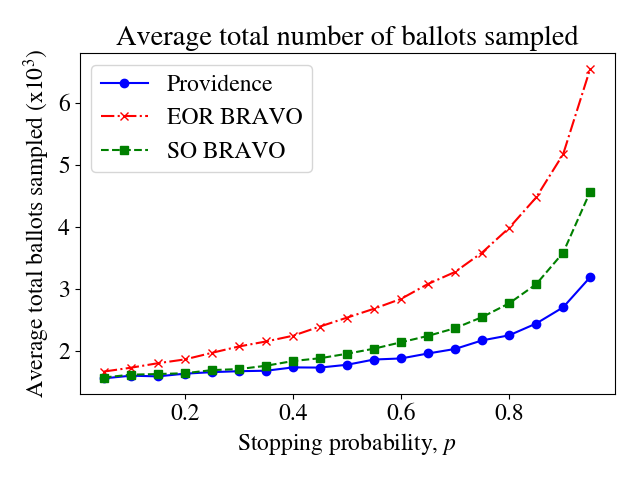
\includegraphics[width=.5\textwidth]{avg_bals.png}
\caption{The total number of ballots sampled on average in our simulations for various round schedules parameterized by $p$ the conditional stopping probability used to select each round size.}
\label{fig:avg_bals}
\end{figure}

\begin{figure}
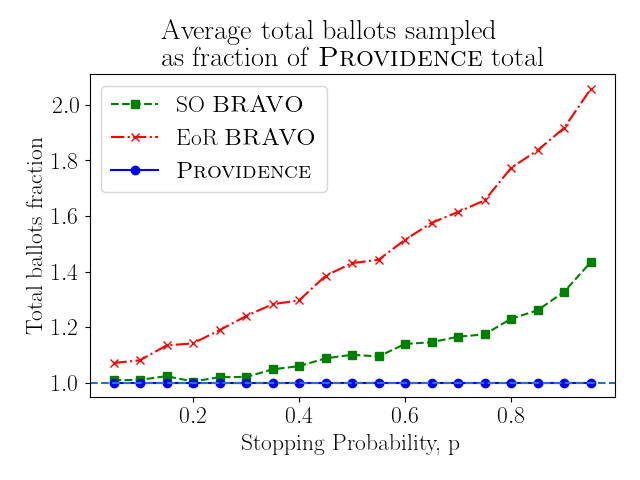
\includegraphics[width=.5\textwidth]{avg_bals_ratio.png}
\caption{The total number of ballots sampled on average in our simulations given as a fraction of those sampled by Providence, for various round schedules parameterized by $p$ the conditional stopping probability used to select each round size.}
\label{fig:avg_bals_ratio}
\end{figure}

It is clear that average number of ballots alone is an inadequate workload measure. 
(Consider a state conducting its audit by selecting a single ballot at random, 
notifying just the county where the ballot is located, and then waiting to hear back for the manual interpretation of the ballot before moving on to the next one. 
This of course is preposterous and is why audits are actually performed in rounds.

In a US state-wide RLA, the state organizes the audit by determining the random sample and communicating with the counties, but election officials at the county level physically sample and inspect the ballots from their precincts. 
Therefore each audit round requires some number of person-hours for set up and communication between state and county. This overhead for a round includes choosing the round size, generating the random sample, and communicating that random sample to the counties, as well as the communication of the results back to the state afterwards. 
%To make it clear that this overhead exists, 

Consequently, we now consider a model with a constant per-ballot cost $c_b$ and a constant per-round cost $c_r$.
So for an audit $\mathcal{A}$ with expected number of ballots $E_{b}$ and expected number of rounds $E_{r}$, we estimate that the cost $C$ of the audit is
\begin{equation}
C(\mathcal{A}) = E_b c_b + E_r c_r
\label{eq:round_cost}
\end{equation}

For simplicity, (and without loss of generality), we assume the per ballot cost is one, $c_b=1$. Then the per round cost $c_r$ tells us the cost of a round as a number of ballots. We begin with $c_r=1000$ as a conservative example. 
That is, we set the overhead of a round equal to the workload of sampling $1000$ ballots. Based on available data[rhode island nums], the time retrieving and analyzing each individual ballot is on the order of $75$ seconds which means that $c_r=1000$ is equivalent to roughly $20$ person-hours of workload. This corresponds to about $15$ minutes being spent per round in each of the $133$ counties of Virginia, a clearly conservative workload estimate. 
As shown in Figure~\ref{fig:with_round_cost}, lower average costs are achieved by selecting higher stopping probability; Providence achieves the lowest minimum average cost is achieved at roughly $0.7$.

\begin{figure}
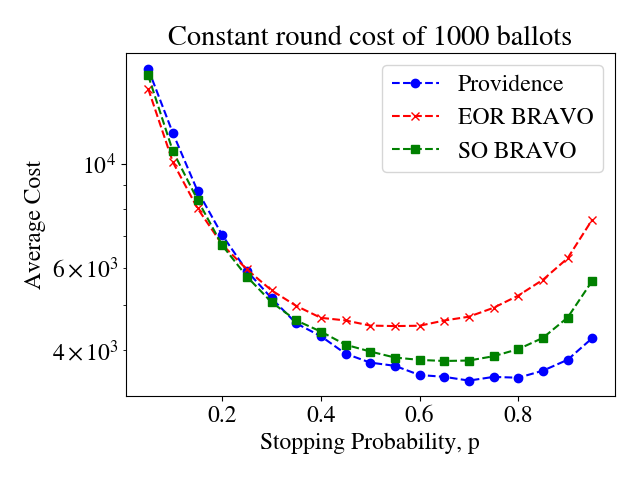
\includegraphics[width=.5\textwidth]{with_round_cost.png}
\caption{For cost parameters $c_b=1$ and $c_r=1000$, this plot shows the expected cost for various round schedule parameters $p$. Expected cost is found using Equation~\ref{eq:cost} and the average number of ballots and rounds in our simulations as the expected number of ballots and rounds.}
\label{fig:with_round_cost}
\end{figure}

Importantly, this gives us a way to estimate the expected cost, as well as which round schedule value $p$ achieves it, for arbitrary round cost. For each round cost $c_r$, we estimate the minimum of the data like that shown in Figure~\ref{fig:with_round_cost} by fitting a lower order polynomial.
Figure~\ref{fig:optimal_costs} shows the optimal achievable workload for a wide range of per round costs. Figure~\ref{fig:optimal_ps} shows the corresponding round schedule parameters $p$ that achieve the minimal workloads. For any reasonable round costs, Providence minimizes cost with at least roughly $10\%$ and $30\%$ improvement over SO BRAVO and EoR BRAVO respectively.

\begin{figure}
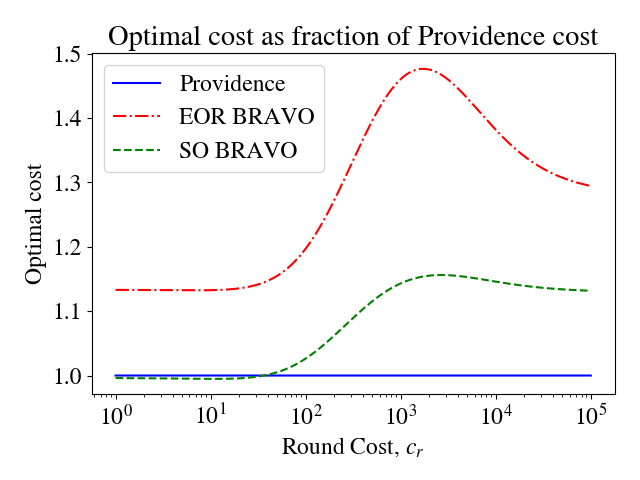
\includegraphics[width=.5\textwidth]{optimal_costs.png}
\caption{For varying round cost $c_r$, the optimal average cost achievable by each audit, as a fraction of the Providence values.}
\label{fig:optimal_costs}
\end{figure}

\begin{figure}
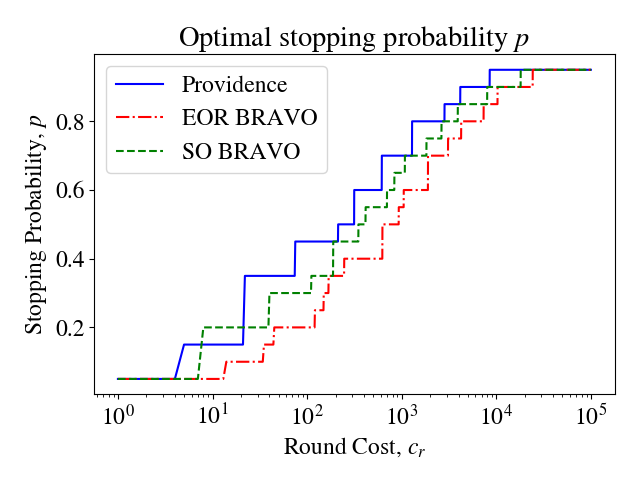
\includegraphics[width=.5\textwidth]{optimal_ps.png}
\caption{The optimal (cost-minimizing) stopping probability $p$ for varying cost model parameters $c_r$. With $c_b=1$, the varying value of $c_r$ can equivalently be thought of as the ratio of the cost of a round to the cost of a ballot.}
\label{fig:optimal_ps}
\end{figure}

Another consideration for election officals is the sensitivit
Election officials may also want to choose larger sample sizes in order to avoid small samples with misleading tallies. In particular, it may be desirable to avoid with very high probability a case in which a sample shows a true loser winning. Assuming a correctly announced outcome, it is straightforward to compute the probability with which a reported loser has more votes than the true winner in a sample, and so we incorporate this into our tool as well. As an illustrating example, our simulations ... TODO

For a more complete model, we can also introduce container-level workload. The time to sample a ballot from an entirely new box is typically much greater than to sample a ballot from an already-open box. [rhode islandd numbers shows it is abou tthis] Available election results give per-precinct granularity of vote tallies, as opposed to individual box informatoin. In Virginia, however, most precincts have a single ballot scanner whose one box has sufficient capacity for the ballots cast in that precinct anyways, and so we model the per-container workload as a per-precinct constant cost, $c_p$. In this model, the workload estimate incurs an additional cost of $c_p$ every time a precinct is sampled from for the first time in a round. That is, let $E_{pi}$ be the expected number of distinct precincts sampled from in round $i$, and let $E_p=\sum_i E_{pi}$. Then the new model is
\begin{equation}
C(E_b, E_r, E_p) = E_b c_b + E_r c_r + E_p c_p
\label{eq:round_and_precinct_cost}
\end{equation}

We can again explore the minimum achievable workloads under this model, as shown in Figure~\ref{fig:optimal_costs_with_precinct}.

\begin{figure}
\includegraphics[width=.5\textwidth]{optimal_costs_with_precinct.png}
\caption{The average cost of the audits we simulated using workload function \ref{eq:round_and_precinct_cost}.}
\label{fig:optimal_ps}
\end{figure}




\subsection{Real time}
Given tight certification deadlines\footnote{Virginia recently passed legislation requiring pre-certification RLAs TODO check exactly.}, the total real time spent is also an important factor to consider when planning audits.

TODO





